\begin{homeworkProblem}
    (5 pts) (Shankar) Exercise 5.2.2 part (a) only

    Exercise 5.2.2* (a) Show that for any normalized $|\psi\rangle$, $\langle\psi|H|\psi\rangle\geq E_0$, where $E_0$ is the lowest-energy eigenvalue. (Hint: Expand $|\psi\rangle$ in the eigenbasis of $H$.)

	\begin{callout}{Solution:}

        \begin{align*}
            \braket{\psi|H|\psi} &= \int_{-\infty}^{\infty} \braket{\psi|H|n}\braket{n|\psi} ~dn \\ 
            &= \int_{-\infty}^{\infty} E_n \braket{\psi | n} \braket{n|\psi} ~dn  \\ 
            &\geq \int_{-\infty}^{\infty} E_0 \braket{\psi|n}\braket{n|\psi} ~dn \\ 
            &\geq E_0 \braket{\psi|\psi} \\ 
            &\geq E_0
        \end{align*}
        
	\end{callout}

\end{homeworkProblem}

\newpage
\begin{homeworkProblem}
    (15 pts) Exercise 5.2.6 (Shankar)

    Exercise 5.2.6* Square Well Potential. Consider a particle in a square well potential:

    \[ V(x) = 
        \begin{cases}
            0, & |x| \leq a \\
            V_0, & |x| > a
        \end{cases} \]

    Since when $V_0 \to \infty$, we have a box, let us guess what the lowering of the walls does to the states. First of all, all the bound states (which alone we are interested in), will have $E \leq V_0$. Second, the wave functions of the low-lying levels will look like those of the particle in a box, with the obvious difference that $\psi$ will not vanish at the walls but instead spill out with an exponential tail. The eigenfunctions will still be even, odd, even, etc.

    \begin{enumerate}[(1)]
        \item Show that the even solutions have energies that satisfy the transcendental equation

            \[ k \tan ka = \kappa \tag{5.2.23} \]

            while the odd ones will have energies that satisfy

            \[ k \cot ka = -\kappa \tag{5.2.24} \]

            where $k$ and $\kappa$ are the real and complex wave numbers inside and outside the well, respectively. Note that $k$ and $\kappa$ are related by

            \[ k^2 + \kappa^2 = 2mV_0/\hbar^2 \tag{5.2.25} \]
            \begin{callout}{Solution (I swap $k$ and $\kappa$):}

                We have the wavefunction
                $$ \frac{\hbar}{2m} \psi'' + V(x)\psi = (E) \psi $$

                \begin{align*}
                    \begin{cases}
                        \psi''(x) &= -k^2\psi, \quad k\equiv \frac{\sqrt{ 2mE }}{\hbar}, \quad \textrm{for}~|x|<a \\ 
                        \psi''(x) &= \kappa^2\psi, \quad \kappa \equiv \frac{\sqrt{ 2m(V_0-E) }}{\hbar}, \quad \textrm{for}~|x|>a \\ 
                    \end{cases}
                \end{align*}

                This gives exponential solutions in Regions $I$ and $III$ where there is a potential, and sin/cos solutions in region $II$.
                \begin{align*}
                    \begin{array}{cl}
                        \ket{\psi_{I}(x)} &= \quad Ae^{-kx} + Be^{kx} \\
                        \ket{\psi_{II}(x)} &= \quad Ce^{-i\kappa x} + De^{i\kappa x} \\ 
                        \ket{\psi_{III}(x} &= \quad Fe^{-kx} + Ge^{kx} \\ 
                    \end{array}
                \end{align*}

                The condition of finiteness demands that $B=G=0$.
                The condition of continuity demands that $\ket{\psi_{I}(-a)} = \ket{\psi_{II}(-a)}$ and $\ket{\psi_{II}(a)}=\ket{\psi_{III}(x(a)}$. This potential is an even function, so we can assume that the solutions are either even or odd.

                \begin{enumerate}[i.]
                    \item \textbf{Even solutions:} 
                        $$\ket{\psi} = \begin{cases}
                            Ae^{-kx}, &\textrm{(x>a)}\\
                            D\cos( \kappa x), &\textrm{(0<x<a)}\\
                            \psi(-x), &\textrm{(x<0)}
                        \end{cases}$$

                        Continuity tells us that 
                        \begin{align*}
                            Fe^{-ka} &= D \cos(\kappa a) \\
                            -Fe^{-ka} &= -D \sin(\kappa a)
                        \end{align*}

                        Dividing the two gives us a relation which allows us to solve for energies:
                        $$k=\kappa \tan (\kappa a)$$

                    \item \textbf{Odd solutions:} 
                        $$\ket{\psi} = \begin{cases}
                            Ae^{-kx}, &\textrm{(x>a)}\\
                            D\sin( \kappa x), &\textrm{(0<x<a)}\\
                            \psi(-x), &\textrm{(x<0)}
                        \end{cases}$$

                        Continuity tells us that 
                        \begin{align*}
                            Fe^{-ka} &= C \sin(\kappa a) \\
                            -Fe^{-ka} &= C \cos(\kappa a)
                        \end{align*}

                        Dividing the two gives us a relation which allows us to solve for energies:
                        $$-k=\kappa \cot (\kappa a)$$


                \end{enumerate}


            \end{callout}

        \item Equations (5.2.23) and (5.2.24) must be solved graphically. In the $(a=ka, \beta)$ plane, imagine a circle that obeys Eq. (5.2.25). The bound states are then given by the intersection of the curve $\alpha \tan \alpha = \beta$ or $\alpha \cot \alpha = -\beta$ with the circle. (Remember $\alpha$ and $\beta$ are positive.)
            \begin{callout}{Solution:}
                
                \begin{align*}
                    k&=\kappa \tan (\kappa a), \qquad \textrm{(even)} \\
                    -k&=\kappa \cot (\kappa a), \qquad \textrm{(odd)}
                \end{align*}

                let 
                $$\left\{\begin{array}{cl}
                    z &=\quad \kappa a \\
                    z' &=\quad k a \\
                    z_0 &=\quad \frac{a}{\hbar} \sqrt{ 2mV_0 } \\
                    z^2 + z_0^2 &=\quad \frac{2ma^2V_0}{\hbar^2}
                \end{array}\right.$$

                Valid energies are given by
                    $$\begin{cases}
                        z' &=\quad z \tan z \\
                        z' &=\quad -z \cot z
                    \end{cases}$$

                    \begin{figure}[H]
                        \centering
                        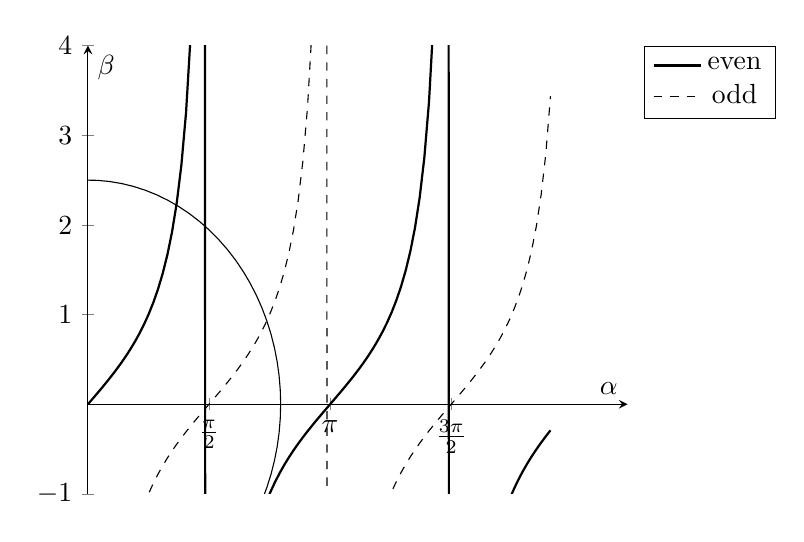
\begin{tikzpicture}
                            \begin{axis}[
                                    domain=0:6.5,
                                    axis x line=middle,
                                    axis y line=middle,
                                    xlabel={$\alpha$},
                                    ylabel={$\beta$},
                                    ymin=-1, ymax=4,
                                    xmin=0, xmax=7,
                                    xtick={pi/2, pi, 3*pi/2},
                                    xticklabels={$ \frac{\pi}{2} $, $ \pi $, $ \frac{3\pi}{2} $},
                                    ytick={-1,0,1,2,3,4},
                                    samples=100,
                                    legend pos=outer north east
                                ]
                                % Plot for odd solutions
                                \addplot[domain=0:6, thick] {tan(deg(x))};
                                \addlegendentry{even}

                                % Plot for even solutions
                                \addplot[domain=0:6, dashed] {-cot(deg(x))};
                                \addlegendentry{odd}

                                % Adding the curve that intersects
                                \addplot[domain=0:360, samples=100] ({2.5*cos(x)}, {2.5*(sin(x)});
                            \end{axis}
                        \end{tikzpicture}
                        \caption{Plot for odd and even solutions of $\beta = \alpha \tan(\alpha)$ and $\beta = -\alpha \cot(\alpha)$}
                    \end{figure}

            \end{callout}
        \item Show that there is always one even solution and that there is no odd solution unless $V_0 > \hbar^2\pi^2/8ma^2$. What is $E$ when $V_0$ just meets this requirement? Note that the general result from Exercise 5.2.2b holds.
            \begin{callout}{Solution:}
                
                Graphically there is always going to be at least 1 intersection between our circle and the odd solution curve, however if the radius of the circle is small enough there may not be a solution for the odd solutions. It happens that when $V_0>\frac{\hbar^2\pi^2}{8ma^2}$ there exist only even solutions.

            \end{callout}

    \end{enumerate}

    Hint: For part (2), make a simple sketch to show the 3 curves (5.2.23-5.2.25). Then, you should be able to solve (3) rather easily by inspecting the figure you draw. (no complicated calculation or precise plotting is needed).
\end{homeworkProblem}

\newpage
\begin{homeworkProblem}
    (5 pts) 3. Exercise 5.3.4 (Shankar)

    Exercise 5.3.4* Consider $\psi = A e^{i\alpha x/\hbar} + B e^{-i\alpha x/\hbar}$ in one dimension. Show that $j = (|A|^2 - |B|^2)\alpha/m$. The absence of cross terms between the right- and left-moving pieces in $\psi$ allows us to associate the two parts of $j$ with corresponding parts of $\psi$.
    \begin{callout}{Solution:}
        
        $j$ refers to the current density of this wave function. In electromagnetism we have the continuity equation which states that any decrease of charge in a volume equals the flow of charge out of it. 
        \begin{align*}
            \frac{\partial \rho}{\partial t} &= - \nabla \cdot \vec{j} \\ 
            \frac{\partial \rho}{\partial t} = i\hbar \frac{\partial \psi^*\psi}{\partial t} &= -\nabla \cdot \vec{j} \\ 
            \frac{\partial \rho}{\partial t} &= - \frac{\hbar}{2mi} \nabla \cdot \left( \psi^* \nabla \psi - \psi \nabla \psi^* \right)
        \end{align*}

        So therefore:
        $$\vec{j} = \frac{\hbar}{2mi}\left( \psi^*\nabla \psi - \psi \nabla \psi^* \right)$$

        \begin{align*}
            \begin{cases}
                \nabla \psi &= \quad A\frac{i \alpha}{\hbar} e ^{i \alpha x / \hbar} - B\frac{i \alpha}{\hbar} e ^{-i \alpha x / \hbar} \\ 
                \nabla \psi^* &= \quad -A\frac{i \alpha}{\hbar} e ^{-i \alpha x / \hbar} + B\frac{i \alpha}{\hbar} e ^{i \alpha x / \hbar} \\
            \end{cases}
        \end{align*}

        \begin{align*}
            \psi^* \nabla \psi &= \left( Ae^{-i \alpha x/\hbar} + Be^{i \alpha x/\hbar} \right) \left( A\frac{i \alpha}{\hbar} e ^{i \alpha x / \hbar} - B\frac{i \alpha}{\hbar} e ^{-i \alpha x / \hbar} \right) \\ 
            &= A^2 \frac{i \alpha }{\hbar} - B^2 \frac{i \alpha}{\hbar} \\ 
            &= \frac{i \alpha }{\hbar} \left( A^2 - B^2 \right) \\ \\
            \psi \nabla \psi^* &= \left( Ae^{i \alpha x / \hbar} + Be^{-i \alpha x / \hbar} \right) \left( -A \frac{i \alpha}{\hbar} e^{-i \alpha x / \hbar} + B \frac{i \alpha}{\hbar} e^{i \alpha x/\hbar} \right) \\ 
            &= - A^2 \frac{i \alpha }{\hbar} + B^2 \frac{i \alpha}{\hbar} \\ 
            &= \frac{i \alpha}{\hbar} (B^2 - A^2)
        \end{align*}

        \begin{align*}
            \vec{j} &= \frac{\hbar}{2mi} \left( \frac{i \alpha}{\hbar} \right)\left( [A^2 - B^2] - [-A^2 + B^2] \right) \\ 
            &= \frac{\cancel{\hbar}}{2m\cancel{i}} \left( \frac{\cancel{i} \alpha}{\cancel{\hbar}} \right)\left( [A^2 - B^2] + [A^2 - B^2] \right) \\ 
            &= \frac{\alpha}{2m} \left( 2[A^2-B^2] \right) \\ 
            &= \frac{\alpha}{m} [|A|^2 - |B|^2]
        \end{align*}

    \end{callout}
\end{homeworkProblem}
